\subsection{Beam Statics}
\label{sec:beam_statics}
\framecard{Beam Statics}



% Set up
\begin{frame}{Set up}
	\txb{120}{3}{12}{
		\begin{block}{Static case }
{			\scriptsize
\begin{itemize}
	\item Support: $\Omega_0 (s=0)$
	\item Crane: $\Omega$\\ axis: $\vct{e}{}{},\pscl{\ebv}{\iz}=\cos\alpha, \pscl{\ebv}{\iy}=\sin\alpha, \alpha\in\psp{0,\frac{\pi}{2}}$\\ geometry: $s\in\left]0,L\right[$, cross-section area $A$,\\ cross-section geometric moment of inertia $\tens{J}{}{}= I \tens{I}{}{}+ \left(J - I\right) \vct{e}{}{}\otimes\vct{e}{}{}$ \\ material properties: $E$, $\mu$\\
	distributed load: $\fv[L]=\zerov$
	\item Rigid horizontal plate $\Omega_p$:\\
	clamping in $\xv[p] (s=L)$, center of mass $\xv[C_m]=\xv[p]+l_x\ix+l_y\iy+l_z\iz$
\end{itemize}              }                                                                              \end{block}
\begin{center}
	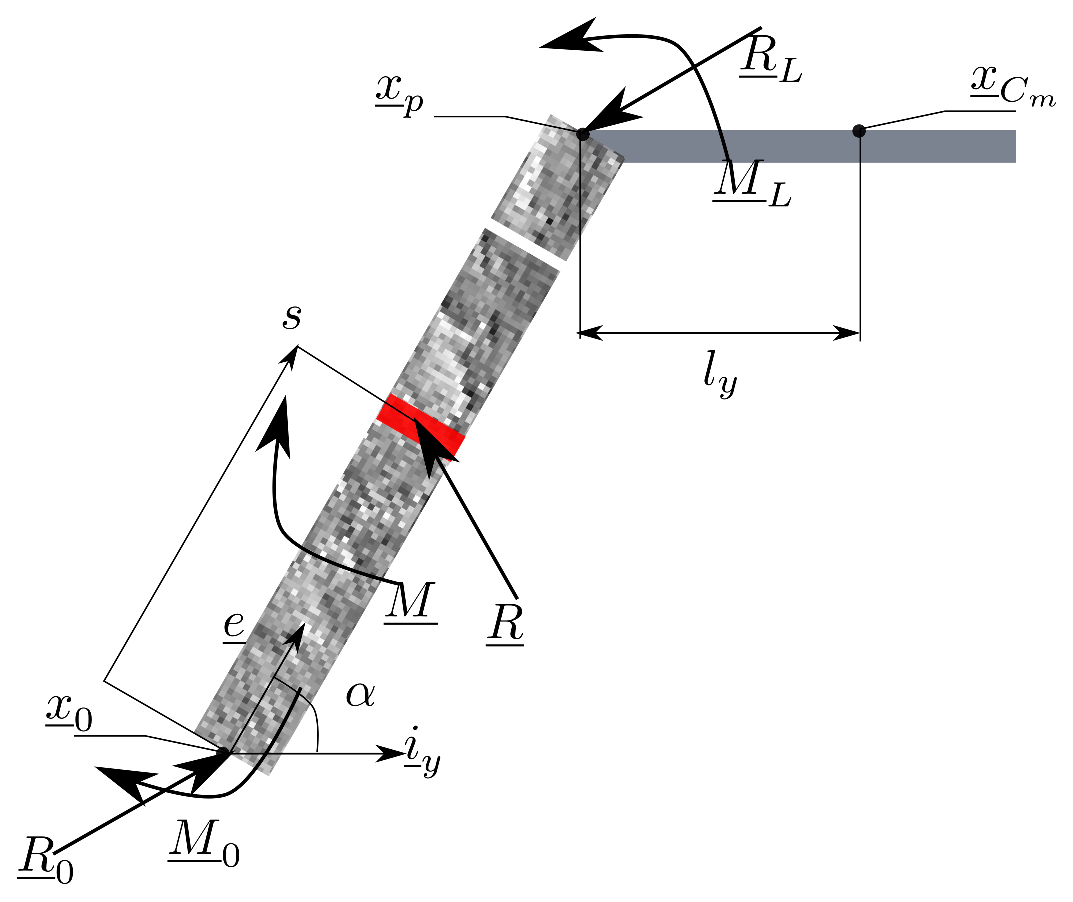
\includegraphics[width=40mm]{moving_crane_1.eps}
\end{center}

	}
\end{frame}
